\documentclass[aspectratio=169]{beamer}
\usepackage{subcaption}
\usepackage{graphicx}  % Required for including images
\usepackage{algorithm}
\usepackage{algpseudocode}
\usepackage{beamerbasetitle}
\usetheme{JuanLesPins}
\usepackage{natbib}
\setbeamertemplate{navigation symbols}{}
\setbeamertemplate{footline}[frame number]

%\setbeamertemplate{headline}{}

\title{Comparative Analysis of Selection Sort and TimSort}
\author
{
  \begin{tabular}[t]{c@{\extracolsep{8mm}}c@{\extracolsep{8mm}}c}
    {\it \small Shahriar Rizvi} & {\it \small Tanvir Mahamood} & {\it \small Rushnan Reaz}\\
    \small Department of CSE & \small Department of CSE & \small Department of CSE\\
    \small RUET & \small RUET & \small RUET\\
    \small 2003104@student.ruet.ac.bd & \small 2003062@student.ruet.ac.bd & \small 2003101@student.ruet.ac.bd\\
    \\
    {\it \small Jaeed Mahmud} & {\it \small Nafees Ahamed} & {\it \small Rakebul Hasan Nur}\\
    \small Department of CSE & \small Department of CSE & \small Department of CSE\\
    \small RUET & \small RUET & \small RUET\\
    \small 2003074@student.ruet.ac.bd & \small 2003079@student.ruet.ac.bd & \small 2003066@student.ruet.ac.bd\\
  \end{tabular}
}
\date{\today}

\begin{document}

\maketitle

\begin{frame}{Title Page}
    \frametitle{Presentation Overview}\tableofcontents
\end{frame}

\section{Abstract}
  \begin{frame}{Abstract}
    \textbf{\fontsize{14}{16}\selectfont Abstract}
    \\This article presents two popular sorting algorithms named Selection Sort and TimSort. The goal of this article is to discuss the sorting techniques, compare their performance with real-life data, and discuss complexity analysis in terms of best-case and worst-case, and space or auxiliary complexity.
    

  \end{frame}

  \section{Introduction}
  \begin{frame}{Introduction}

    \textbf{\fontsize{14}{16}\selectfont Introduction}
    \\Selection Sort is akin to a brute force approach, while Tim Sort employs a divide-and-conquer strategy by incorporating merge sort.\\
    Selection sort is a sorting algorithm that selects the smallest element from an unsorted list in each iteration and places that element at the beginning of the unsorted list. Tim Sort is a hybrid algorithm modified from merge sort and insertion sort. It was designed to perform real-life operations. Tim Sort is the default sorting algorithm used by Python’s sorted() and list.sort() functions.\\

  \end{frame}


  \section{Background Study}
   \subsection{Selection Sort}
 \begin{frame}{Background Study: Selection Sort}   
    \textbf{\fontsize{14}{16}\selectfont Selection Sort}
    \begin{itemize}
        \item Selection Sort\citep{Knuth-Selection} is a straightforward but inefficient algorithm used for sorting arrays.
        \item The main idea is to find the smallest element in the array and move it to the front, repeating this process until the array is sorted.
         \item This algorithm involves a linear search to find the smallest element and utilizes swapping to rearrange the elements
    \end{itemize}

  \end{frame}
\subsubsection{Algorithm}
  \begin{frame}{Algorithm}
    
  \begin{algorithm}[H]
    \caption{Selection Sort}
    \begin{algorithmic}[1]
      \Procedure{SelectionSort}{$A, n$} \Comment{A is the array to be sorted, n is the size of the array}
      \For{$i \gets 0$ \textbf{to} $n-1$}
      \State $minIndex \gets i$
      \For{$j \gets i+1$ \textbf{to} $n$}
      \If{$A[j] < A[minIndex]$}
      \State $minIndex \gets j$
      \EndIf
      \EndFor
      \State Swap $A[i]$ and $A[minIndex]$
      \EndFor
      \EndProcedure
    \end{algorithmic}
  \end{algorithm}
\end{frame}
\subsubsection{Worst Case Analysis}
  \begin{frame}{Worst Case Analysis}
  
    \textbf{Total Complexity}: $c_1 n + c_2(n-1) + c_3n(n-1) / 2 + c_4(n-1) + c_5(n-1) + c_6(n-1) + c_7(n-1)$\\

    \textbf{Worst case:} 
\begin{itemize}

  \item  This case can be achieved when we need to sort an array in ascending order, but the array is initially in descending order. This uses a 'Swap' operation at every iteration.
 So, the overall time cost:
\begin{align*}\setlength{}{}
    T(n) &= c_1n + c_2(n-1) + \frac{c_3n(n-1)}{2} + c_4(n-1)+ c_5(n-1) + c_6(n-1) + c_7(n-1) \\
         &\quad= \frac{c_3}{2}n^2 + (c_1+c_2-\frac{c_3}{2}+c_4+c_5+c_6+c_7) - (c_2+c_4+c_5+c_6+c_7)
\end{align*}

This running time can be expressed as\\ $T(n) = an^2 + bn + c$

  Here, \( a = \frac{c_3}{2} \), \( b = c_1 + c_2 - \frac{c_3}{2} + c_4 + c_5 + c_6 + c_7 \), and \( c = -c_2 - c_4 - c_5 - c_6 - c_7 \).

    \textbf{Complexity:} O($n^2$)\\
\end{itemize}
\end{frame}

\subsubsection{Best Case Analysis}
\begin{frame}{Best Case Analysis}
    
    \begin{itemize}
  \item \textbf{Best case:} Best case happens when the array is already sorted in ascending order as wanted. That time, no swap operation was needed during the total iterations.\\
 Thus, the total time cost will be reduced slightly. That is:\\
 \begin{align*}
  T(n) & = c_1n + c_2(n-1) + c_3n(n-1) / 2 + c_4(n-1)\\
     &\quad= (c_3/2)n^2 + (c_1+c_2-c_3/2+c_4)n + (-c_2-c_4)\\
\end{align*}
   
       This running time can be expressed as \\
$T(n) = a’n^2 + b’n + c’$
Here, $a’ = c_3/2, b = c_1+c_2-c_3/2+c_4$ and $c = -c_2-c_4$.
  \end{itemize}
  \textbf{Complexity:} O($n^2$)

  \end{frame}

  \begin{frame}{Background Study}
  \frametitle{Space Complexity and Stability}
\subsubsection{Space Complexity and Stability}

\textbf{Space Complexity:} As no extra space is needed to sort the array except the ‘Temp’ variable for swapping, the space complexity is O(1).\\  
\vspace{.2cm}
\textbf{Stability:} Selection Sort is an unstable sort.

  \end{frame}


\begin{frame}{Example - Initial Array And Passes}
  \[ A = [64, 25, 12, 22, 11] \]
  %\textbf{\fontsize{13}{13}All Passes}
  \begin{align*}
      After First Pass:  A &= [11, 25, 12, 22, 64] \\
      After Second Pass: A &= [11, 12, 25, 22, 64] \\
      After Third Pass:  A &= [11, 12, 22, 25, 64] \\
      After Fourth Pass: A &= [11, 12, 22, 25, 64] \\
  \end{align*}
\end{frame}

  
   \subsection{TimSort}
  \begin{frame}{Background Study: TimSort}
      \textbf{\fontsize{13}{13}\selectfont Tim Sort}\newline
   
    
      \begin{itemize}
          \item TimSort, a hybrid sorting algorithm invented by Tim Peters in 2002\citep{peters2015TimSort}.
          \item Designed mainly addressing real-world data concerns.
          \item It is derived by modifying Merge Sort\citep{Knuth-Merge} by involving Insertion Sort\citep{Knuth-StInsertion} to perform an optimized sorting algorithm.
          \item Python uses the refined verion proposed by \citet{gouw-java}, Java uses the initial TimSort version with tuning values\citep{Auger-2019}. GNU Octave and Android OS  also use TimSort as the default sorting algorithm.
      \end{itemize}

  \end{frame}
  
  \subsubsection{Algorithm}
\begin{frame}{Algorithm}
  \begin{algorithm}[H]
    \caption{Tim Sort}
    \begin{algorithmic}[1]
      \Procedure{TimSort}{$A, n$}
        \State Calculate and divide $A$ into small min\_runs\footnote{min\_runs are small subsets of $A$ for which the Insertion Sort will perform in best complexity. As stated by \citet{peters2015TimSort} min\_run should range from 32 to 64 elements}.
        \State Perform insertion sort on each min\_run.
        \State Merge min\_runs using modified merge sort. Collapse Runs until a single run is formed.
      \EndProcedure
    \end{algorithmic}
  \end{algorithm}
\end{frame}


  
\subsubsection{Complexities and Stablities}
\begin{frame}{Complexities and Stablities}
 \begin{itemize}
    \item Best Case Complexity: $O(n)$ - Array is already sorted.
    \item Worst Case Complexity: $O(n\log(n))$ - which was firstly proven in the works of \cite{Auger-2015,Auger-2019}.

    \item Auxiliary Space Complexity: $O(n)$ - Additional space for temporary storage and data structures.Uses auxiliary arrays and may employ a stack.
  \item Stable algorithm: Preserves relative order of equal elements. Merging mechanism and Insertion Sort maintain stability.
  \end{itemize}
\end{frame}

\begin{frame}{The Concept of Run}
    \begin{itemize}
        \item \textbf{Definition of a Run:} A run is a contiguous subsequence of elements in an array with a specific order.
        \item Runs can be classified as either:
            \begin{itemize}
                \item \textbf{Ascending Run:} Elements are non-decreasing (\(a_0 \leq a_1 \leq a_2 \leq \ldots\)).
                \item \textbf{Descending Run:} Elements are strictly decreasing (\(a_0 > a_1 > a_2 > \ldots\)).
    \end{itemize}
     \end{itemize}
\textbf{Efficiency in TimSort:}
  \begin{itemize}
    \item Runs contribute to the efficiency of TimSort by minimizing unnecessary operations.
    \item In random data, runs tend to be of length 'min\_run', leading to balanced merges.
    \item In \citet{peters2015TimSort} suggests run should be strictly ascending. 
    \item In the best-case scenario, the array is already sorted and the entire array will work as run.
  \end{itemize}

\end{frame}

  
%  \begin{frame}{The concept of 'Run'}
%       It is clear that the Runs do not need any sorting algorithm. All the Runs and other smallest subarrays are %merged. Thus the value of x is maximised and overall complexity is improved.\newline\\
%       In the best case scenario, the array is already sorted and the entire array will work as ‘Run’. So, we do not %need to take a divide and conquer approach. Simply the Time complexity is O(n).
%        In the worst case scenario, the Time complexity is O($n\log(n)$). Because all the operations from divide and %%    \end{frame}
    \section{Results and Analysis}
    
    \begin{frame}{Results and Analysis}
    
    
    \textbf{\fontsize{14}{16}\selectfont Results and Analysis}\newline

    In this section, we present the results of our time analysis comparing Selection Sort and Tim Sort on datasets of different sizes (900, 9000, and 100000 data points). Additionally, we include visualizations of the theoretical time complexities represented by \(O(n^2)\) and \(O(n \log n)\) graphs for reference.\\
  \end{frame}

  \begin{frame}{Time Analysis}
      %\textbf{Time Analysis}\newline
      We conducted a comprehensive time analysis to assess the performance of Selection Sort and Tim Sort across varying dataset sizes. The results are illustrated in Figures \ref{d900}, \ref{d9k}, and \ref{d100k} for dataset sizes of 900, 9000, and 100000 data points, respectively.
      \begin{figure}
	\centering
	\begin{subfigure}{\textwidth}
		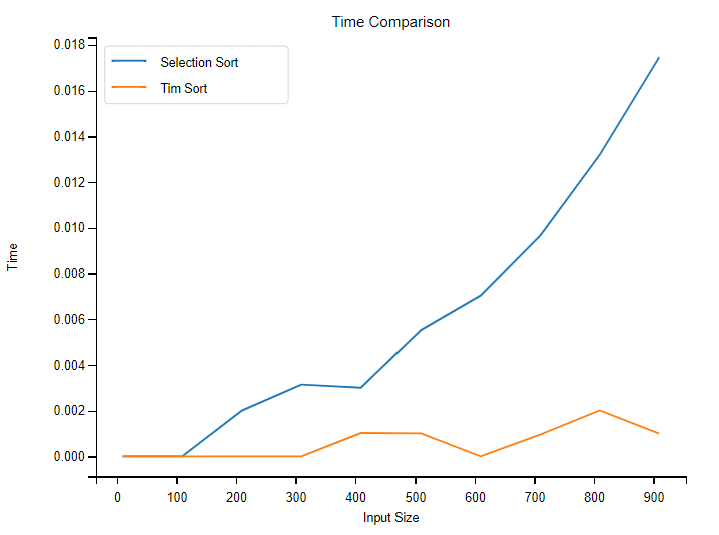
\includegraphics[scale=0.25]{Images/900_time_comp.png}
		\caption{For data size: 900}
		\label{d900}
	\end{subfigure}
	\caption{Time Comparison between Selection and Tim Sort(900)}
        \end{figure}
  \end{frame}

    \begin{frame}{Comparison Graph}
    
        
    
        \begin{figure}
    \centering
    \begin{subfigure}{\textwidth}
		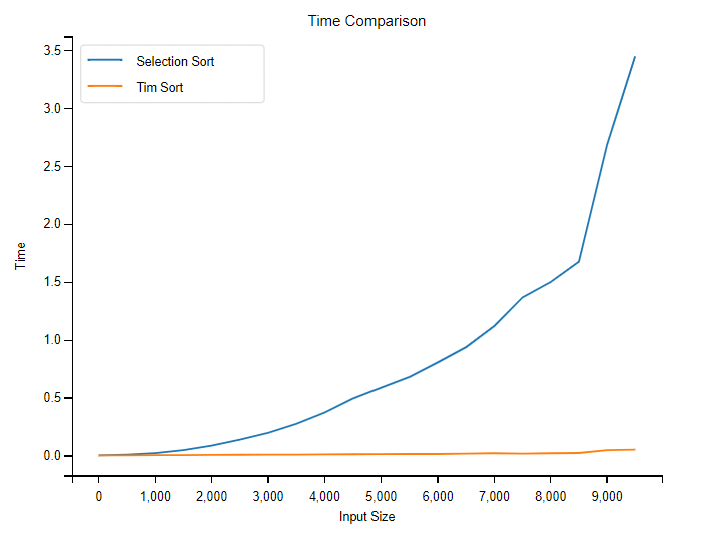
\includegraphics[scale=0.25]{Images/9k_time_comp.png}
		\caption{For data size: 9000}
		\label{d9k}
	\end{subfigure}
        \caption{Time Comparison between Selection and Tim Sort(9000)}
        \end{figure}
       
    \end{frame}

    \begin{frame}{Comparison Graph}
    \begin{figure}[h]
    \centering
    \begin{subfigure}{\textwidth}
		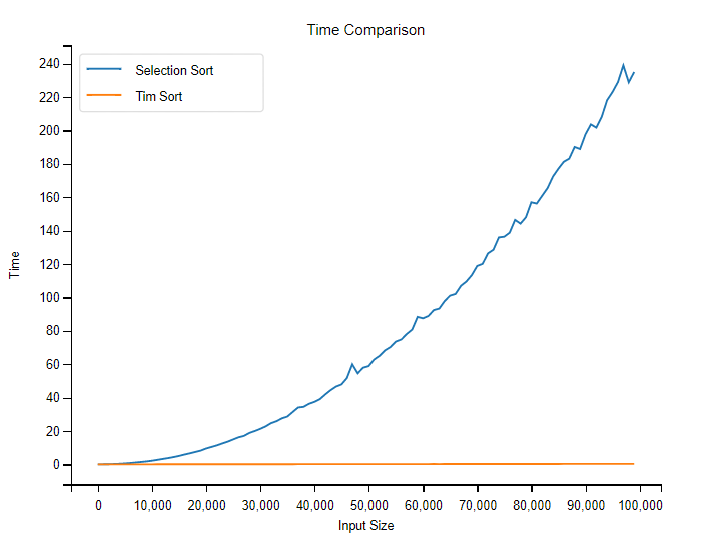
\includegraphics[scale=0.25]{Images/100k_time_comp.png}
		\caption{For data size: 100,000}
		\label{d100k}
	\end{subfigure}
        \caption{Time Comparison between Selection and Tim Sort(100 000)}
        \end{figure}    
    \end{frame}

    
    \begin{frame}{Theoretical Time Complexities}
        As depicted in the figures, Tim Sort consistently outperforms Selection Sort across all dataset sizes. The divide-and-conquer strategy employed by Tim Sort demonstrates its efficiency, particularly as the dataset size increases.\\    
        To provide a theoretical context for our empirical findings, we include graphs representing the time complexities of \(O(n^2)\) and \(O(n \log n)\) in this figure below:
    \\
    \begin{figure}[h]
  \centering
  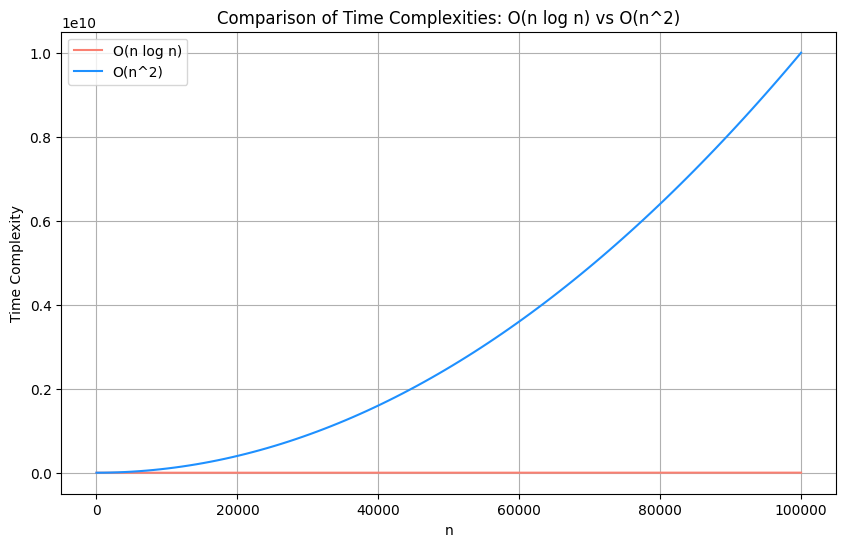
\includegraphics[width=0.5\textwidth]{Images/actual_Function.png}
  \caption{Theoretical time complexities: \(O(n^2)\) and \(O(n \log n)\).}
  \label{fig:theoretical_complexities}
\end{figure}
    \end{frame}
    \begin{frame}{Theoretical Time Complexities}
    The theoretical complexities serve as a reference point, confirming that the observed performance aligns with the expected behaviors of Selection Sort and Tim Sort.\newline

In summary, our empirical results and theoretical considerations collectively suggest that Tim Sort is a more efficient sorting algorithm compared to Selection Sort, especially in scenarios with larger.\newline\\
    \end{frame}

    \begin{frame}{Comparison}
   
    \begin{itemize}
	\item TimSort is very optimized. Its best-case and worst-case time complexity is O(n) and O($n\log(n)$) respectively. On the other hand, Selection Sort is very inefficient and runs in O($n^2$) for both worst and best cases.
	\item Selection Sort uses no extra space for sorting. It is space-optimized. TimSort is not space-optimized.
	\item TimSort is a stable sorting algorithm. Selection Sort is unstable.
    \end{itemize}
        
    \end{frame}
      \section{Conclusion}
    \begin{frame}{Conclusion}
  
    \textbf{\fontsize{14}{16}\selectfont Conclusion}\newline
    This paper represents two sorting algorithms (Selection Sort and TimSort), their sorting techniques, time complexity, and performance. To compare sorting algorithms, the time complexity is the main consideration.\newline
     It upholds the comparison of performance by graph, which highlights the high efficiency of TimSort for a large number of elements that are to be sorted.\newline
     \\So, We can say that for any case Timsort is better than Selection Sort but in terms of space complexity Selection Sort is better as it consumes less coding space.
    
\end{frame}

    \section*{ }
    \begin{frame}[t]
    
        \frametitle{References}
        \centering
        \small
        \bibliographystyle{plainnat}
        \bibliography{mybib2}
    \end{frame}

\begin{frame}{Contribution}
    \begin{itemize}
        \item Paper Writing:\\
        Tanvir Mahamood(2003062)\\
        Jaeed Mahmud(2003074)\\\newline
        \item Paper Formatting:\\
        Shahriar Rizvi(2003104)\\
        Rushnan Reaz(2003101)\\\newline
        \item Slide Preparation:\\
        Rakebul Hasan Nur(2003066)\\
        Nafees Ahamed(2003079)
    \end{itemize}
 
    
    \begin{center}
        \textbf{Thank You}
    \end{center}
\end{frame}
    

\end{document}